\documentclass[10pt,letterpaper]{article}
\usepackage[left=1.8cm, right=1.8cm, top=1cm]{geometry}
\usepackage[utf8]{inputenc}
\usepackage[T1]{fontenc}
\usepackage[spanish]{babel}
\usepackage{amsmath}
\usepackage{amsfonts}
\usepackage{amssymb}
\usepackage{graphicx}
\usepackage{subfigure}
\usepackage{steinmetz}
\usepackage{float}
%\usepackage{circuitikz}

\author{Clase Práctica $\#$1}
\title{Electrónica I}
\date{Componentes básicos y leyes de tensión y corriente}

\renewcommand{\sin}{\sen}
\begin{document}
	\maketitle
	
%	Temas
%	\begin{itemize}
%		\item Leyes de Kirchhoff.
%		\item Combinaciones de resistencias.
%		\item Fuentes reales.
%		\item Potencia.
%	\end{itemize} 

Bibliografía: Análisis de circuitos en ingeniería. Hayt \textit{et al.} 8va ed. Capítulos 2 y 3
\\

	
 1- En el circuito que se muestra en la figura, los valores de las resitencias son desconocidos, pero se sabe que la fuente de 2 $\mathrm{V}$ suministra una corriente de 7 $\mathrm{A}$ al resto del circuito. Calcule la corriente etiquetada como $i_2$.

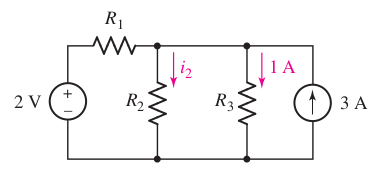
\includegraphics[width=.5\linewidth]{ej1}	

2- Determine un valor numérico para cada corriente y tensión ($i_1$ , $v_1$ , etc.) en el circuito de la figura:

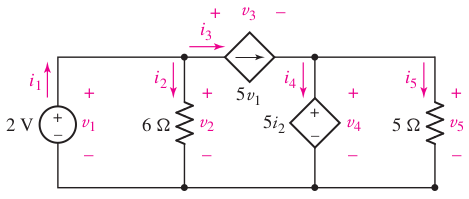
\includegraphics[width=.5\linewidth]{ej2}	
%\pagebreak

3- Haciendo un uso apropiado de las técnicas de combinación de resistencias, calcule $i_3$ en el circuito de la figura y la potencia suministrada al circuito por la fuente de corriente.

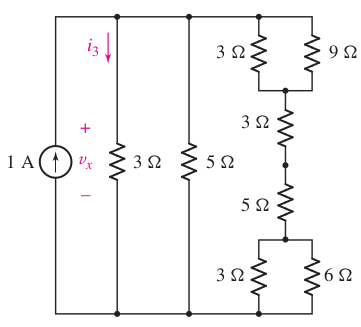
\includegraphics[width=.45\linewidth]{ej3}

4- El circuito muestra una fuente de voltaje real a la cual se le ha conectado una carga $R_L$.

	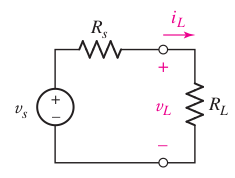
\includegraphics[width=.3\linewidth]{c4}

a) A partir de un valor de $R_s$ obtenga el valor de $R_L$ para la cual la transferencia de potencia sea máxima así como dicha potencia.
\\
%b) Suponga que la corriente a través de $R_L$ tiene una forma de onda sinusoidal con una amplitud máxima de  $100~\mathrm{mA}$. Si $R_L=1~\mathrm{k}\Omega$ calcule la potencia promedio disipada en el resistor.

%\textbf{Comentarios}. en el a) es escribir la potencia y derivarla por $R_L$ para obtener $R_L=R_s$ y $P=\dfrac{V_s^2}{4R_s}$.
%
%El b va por la idea de mostrar la diferencia entre potencia promedio e instantánea, además del concepto de valor eficaz o efectivo de la corriente / voltaje. 

5- En el circuito de la figura, sólo interesa la tensión $v_x$ . Simplifique el circuito usando la combinación adecuada de resistencias y empleando iterativamente división de tensión para determinar $v_x$

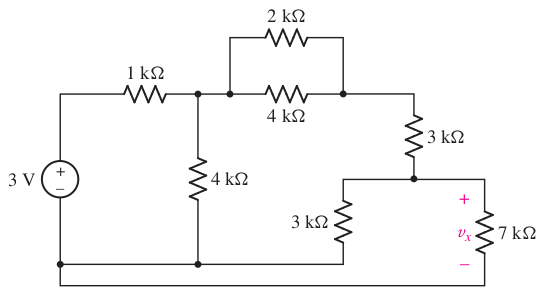
\includegraphics[width=.5\linewidth]{ej5}

%\pagebreak

6- Calcule la tensión marcada como $v_x$ en el circuito de la figura después de simplificar primero, usando combinaciones adecuadas de fuentes y resistencias.

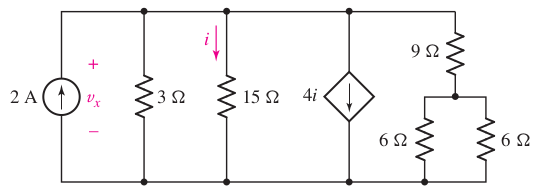
\includegraphics[width=.5\linewidth]{ej6}
\end{document}